 \documentclass{article}
 
 \usepackage{fancyhdr}
 \usepackage{cmap}
 \usepackage[T2A]{fontenc}
 \usepackage[utf8]{inputenc}
 \usepackage[english,russian,ukrainian]{babel}
 \usepackage{pythontex}
 \usepackage{indentfirst}
 \usepackage{graphicx}
 \usepackage{hyperref}
 \hypersetup{
 	colorlinks,
 	citecolor=black,
 	linkcolor=black,
 	filecolor=black,
 	urlcolor=black
 }
 
 \usepackage{geometry}
 \geometry{
 	a4paper,
 	total={165mm,247mm},
 	left=20mm,
 	top=30mm,
 }
 \usepackage{titlesec}
 \usepackage{fancyhdr}
 
 \pagestyle{fancy}
 \fancyhf{}
 \renewcommand{\headrulewidth}{0.5pt}
 \renewcommand{\footrulewidth}{0.5pt}
 \rhead{\LaTeX}
 \lhead{Вячеслав Козачок}
 
 %\titleformat{\section}
 %{\normalfont\Large\bfseries}{\thesection}{1em}{}
 
 %\titleformat*{\subsection}{\large\bfseries}
 
 
 
 \begin{document}
 	
	\begin{titlepage}
	
	\begin{frame}[t]
		\raisebox{-10mm}[10pt][0pt]{%
			\makebox[\textwidth][c]{
\includegraphics[width=\textwidth]{institute.jpg}}
		}
	\end{frame}\\
	\large
	\centering{
		\vspace{5mm}\\
		Міністерство освіти і науки України \\
		Національний технічний університет України \\
		"Київський політехнічний інститут імені Ігоря Сікорського"\\
		Фізико-технічний інститут
	}
	\vspace{3cm}\\
	\centering{
		{\Huge\textbf{Операційні системи} \\ \vspace{0.15cm}}
		{\huge Лабораторна №9}
	}
	
	\vspace{8cm}
	\Large
	\begin{flushright}
		Виконав:\\
		Студент групи ФБ-82\\
		\textbf{Козачок Вячеслав}\\
		Перевірив: \\
		Кіреєнко О.В.
	\end{flushright}
	\vfill
	
	\centering{Київ - 2020}
	
\end{titlepage}
	\newpage
	\Large
	\section{Варіант}
	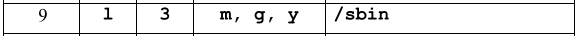
\includegraphics{prot.png}
	\section*{Завдання до виконання}
	\large
	\begin{enumerate}
		\item Перейдіть у каталог\verb|/bin| Перегляньте список усіх файлів, що
		починаються із символу, який визначено в таблиці індивідуальних
		завдань.
		\item Перегляньте список файлів, імена яких складаються з визначеної у
		таблиці індивідуальних завдань кількості символів.
		\item Перегляньте список файлів, імена яких починаються із символів, які
		визначено в таблиці індивідуальних завдань. Зробіть це декількома
		способами.
		\item Створіть у вашому домашньому каталозі підкаталог \verb|lab_4| і перейдіть
		в нього.
		
		\item За допомогою команди \verb|cat| створіть файл \verb|my_text| і запишіть у
		нього кілька рядків. Потім за допомогою команди \verb|cat| допишіть у
		нього ще кілька рядків.
		
		\item Підрахуйте кількість файлів у каталозі, визначеному з таблиці
		індивідуальних завдань, використовуючи і не використовуючи
		конвеєри. Порівняйте результат.
		
		\item Підрахуйте кількість файлів у каталозі, визначеному з таблиці
		індивідуальних завдань, при цьому зберігши список файлів у файлі
		\texttt{filelist}, використовуючи команду \texttt{tee}.
		
		\item Починаючи з вашого домашнього каталогу, виведіть на екран у
		повному форматі назви усіх файлів і каталогів, що починаються з ‘m’.
		При цьому перед виведенням кожної назви на екран повинен
		виводитися запит на його підтвердження.
		
		\item Починаючи з кореневого каталогу, виведіть на екран імена всіх
		каталогів, що останній раз змінювалися більше 15 днів назад.
		
		\item Виведіть на екран тільки час, що повертається командою \texttt{date}.
		
		\item Виведіть на екран список усіх користувачів системи, тобто перші поля
		кожного рядка файлу \texttt{/etc/passwd} (роздільник полів — символ ‘:’).
		
		\item Виведіть на екран імена усіх файлів у каталозі \texttt{/bin}, що містять слова
		Software чи software. Потік помилок при цьому не повинний
		виводитися на екран.
		Увага!!! у цьому завданні мова йде про те, що слова Software чи
		software містяться не у назві файлу (таких файлів там не повинно
		бути), а у самому файлі (а таких файлів має бути достатньо).
		
		\item Відсортуйте конфігураційний файл вашої оболонки (\texttt{.profileprofile} ,
\\
		\texttt{.profilecshrc)} відповідно до кодової таблиці ASCII так, щоб при цьому
		ігнорувалися пробіли на початку рядків. Робіть це з копією файлу,
		щоби не порушити нормальну працездатність вашої оболонки.
		
	\end{enumerate}
	\newpage
	\begin{enumerate}
		\item \begin{verbatim} [eski@eski-pc bin]$ find . -maxdepth 1 -type f | cut -d/ -f2 | grep ^l
		lou_debug
		lvm
		lv2_validate
		localedef
		ldbrename
		.......
		ldns-gen-zone
		lnstat
		libglade-convert
		lit2epub
		lavtc.sh
		lircd-setup
		line-stipple-wide
		\end{verbatim}
		\item 
		\begin{verbatim}
		[eski@eski-pc bin]$ find . -maxdepth 1 -type f -name "???" | cut -d/ -f2 
		gcc
		tie
		lvm
		arp
		ldd
		lz4
		xsd
		gdb
		jiv
		psl
		....
		\end{verbatim}
		
		\item \begin{verbatim}
		[eski@eski-pc bin]$ find . -maxdepth 1 -type f -name "[m,g,y]*" | cut -d/ -f2    
		gsraytrace
		gcc
		mtp-newplaylist
		gloss
		gst-play-1.0
		glxswapcontrol
		groffer
		gtk-query-immodules-3.0
		gdb
		.......
		\end{verbatim}
		
		\item \begin{verbatim}
		[eski@eski-pc bin]$ cd ~
		[eski@eski-pc ~]$ mkdir lab_4
		[eski@eski-pc ~]$ cd lab_4/
		\end{verbatim}
		
		\item
		\begin{verbatim}
		[eski@eski-pc lab_4]$ cat > my_text
		Hello World 
		[eski@eski-pc lab_4]$ cat my_text 
		Hello World 
		[eski@eski-pc lab_4]$ cat >> my_text
		It's real trouble!
		[eski@eski-pc lab_4]$ cat my_text 
		Hello World 
		It's real trouble!
		\end{verbatim}
		
		\item \begin{verbatim}
		[eski@eski-pc sbin]$ find . -maxdepth 1 -type f | wc -l 
		3912
		
		[eski@eski-pc sbin]$ find . -maxdepth 1 -type f > ~/lab_4/files_sbin; 
		cat -b ~/lab_4/files_sbi&
		n > ~/lab_4/count_sbin; 
		tail ~/lab_4/count_sbin
		3903  ./pppd
		3904  ./pactree
		3905  ./jack_bufsize
		3906  ./bg5latex
		3907  ./xxd
		3908  ./pkaction
		3909  ./rdjpgcom
		3910  ./jupyter-console
		3911  ./csc
		3912  ./glsync32
		
		\end{verbatim}
		\item \begin{verbatim}
		[eski@eski-pc sbin]$ find . -maxdepth 1 -type f | cut -d/ -f2 | tee ~/lab_4/files_sbin | wc -l 
		3912
		
		[eski@eski-pc sbin]$ tail ~/lab_4/files_sbin 
		pppd
		pactree
		jack_bufsize
		bg5latex
		xxd
		pkaction
		rdjpgcom
		jupyter-console
		csc
		glsync32
		\end{verbatim}
		
		\small
		\item \begin{verbatim}
		[eski@eski-pc ~]$ find . -name "m*" -print -ok ls -l -d {} \;
		./.IdeaIC2019.2/system/index/stubs/markdown.header
		< ls ... ./.IdeaIC2019.2/system/index/stubs/markdown.header > ? y
		drwxr-xr-x 2 eski eski 4096 Nov 14 00:39 ./.IdeaIC2019.2/system/index/stubs/markdown.header
		./.IdeaIC2019.2/system/index/stubs/markdown.header/markdown.header.storage
		< ls ... ./.IdeaIC2019.2/system/index/stubs/markdown.header/markdown.header.storage > ? y
		-rw-r--r-- 1 eski eski 4096 Nov 14 00:39 ./.IdeaIC2019.2/system/index/stubs/markdown.header
		/markdown.header.storage
		./.IdeaIC2019.2/system/index/stubs/markdown.header/markdown.header.storage.len
		< ls ... ./.IdeaIC2019.2/system/index/stubs/markdown.header/markdown.header.storage.len > ? y
		-rw-r--r-- 1 eski eski 8 Nov 14 00:39 ./.IdeaIC2019.2/system/index/stubs/markdown.header/
		markdown.header.storage.len
		./.IdeaIC2019.2/system/index/stubs/.versions/markdown.header.ver
		< ls ... ./.IdeaIC2019.2/system/index/stubs/.versions/markdown.header.ver > ? ^C
		\end{verbatim}
		\large
		\item \begin{verbatim}
		[eski@eski-pc ~]$ sudo find / -maxdepth 4 -atime 15 -type d
		[sudo] password for eski: 
		find: ‘/run/user/1000/doc’: Permission denied
		find: ‘/run/user/1000/gvfs’: Permission denied
		/home/eski/vmware/tgstat
		/home/eski/vmware/64bit
		/home/eski/vmware/Ubuntu 64-bit
		/var/spool/atd
		/usr/share/doc/at
		/usr/lib/erlang/erts-10.6.2
		\end{verbatim}
		
		\item 
		\begin{verbatim}
		[eski@eski-pc ~]$ date +%d-%m-%H
		27-02-19
		\end{verbatim}
		\item \begin{verbatim}
		[eski@eski-pc ~]$ cat /etc/passwd | cut -d: -f1 | tail
		rtkit
		sddm
		usbmux
		eski
		airflow
		tss
		postgres
		rabbitmq
		mysql
		topshop
		
		\end{verbatim}
		\small
		\item\begin{verbatim}
		[eski@eski-pc bin]$ grep -nwri . -e "software" > ~/lab_4/grep_bin 2> ~/lab_4/grep_error
		
		[eski@eski-pc lab_4]$ ls
		count_sbin  files_sbin  grep_bin  grep_error  my_text
		
		[eski@eski-pc lab_4]$ tail grep_bin 
		./pdfmom:14:# Software Foundation, either version 3 of the License, or
		./lavtc.sh:8:# This program is free software; you can redistribute it and/or modify
		./lavtc.sh:10:# the Free Software Foundation; either version 2 of the License, or
		./lavtc.sh:19:# along with this program; if not, write to the Free Software
		Binary file ./sntp matches
		Binary file ./pppd matches
		./bg5latex:5:# This program is free software; you can redistribute it and/or modify
		./bg5latex:7:# the Free Software Foundation; either version 2 of the License, or
		./bg5latex:17:# Software Foundation, Inc., 51 Franklin St, Fifth Floor, Boston,
		Binary file ./pkaction matches
		
		[eski@eski-pc lab_4]$ tail grep_error 
		grep: ./augenrules: Permission denied
		grep: ./audispd: Permission denied
		grep: ./cupsd: Permission denied
		grep: ./mount.nfs: Permission denied
		
		\end{verbatim}
		
		\newpage
		\item\begin{verbatim}	
		[eski@eski-pc lab_4]$ LC_ALL=C sort -b .bashrc | sed '/^$/d' 
		#
		#
		#
		# # ex - archive extractor
		# # usage: ex <file>
		# Bash won't get SIGWINCH if another process is in the foreground.
		# Change the window title of X terminals
		# Enable checkwinsize so that bash will check the terminal size when
		# Enable colors for ls, etc.  Prefer ~/.dir_colors #64489
		# Enable history appending instead of overwriting.  #139609
		# Set colorful PS1 only on colorful terminals.
		# background colors
		# dircolors --print-database uses its own built-in database
		# export QT_SELECT=4
		# first to take advantage of user additions.  Use internal bash
		# foreground colors
		# globbing instead of external grep binary.
		# http://cnswww.cns.cwru.edu/~chet/bash/FAQ (E11)
		# instead of using /etc/DIR_COLORS.  Try to use the external file
		# it regains control.  #65623
		# show root@ when we don't have colors
		# ~/.bashrc
		&& match_lhs=$(dircolors --print-database)
		&& type -P dircolors >/dev/null \
		*)           echo "'$1' cannot be extracted via ex()" ;;
		*.7z)        7z x $1      ;;
		*.Z)         uncompress $1;;
		*.bz2)       bunzip2 $1   ;;
		*.gz)        gunzip $1    ;;
		*.rar)       unrar x $1     ;;
		*.tar)       tar xf $1    ;;
		*.tar.bz2)   tar xjf $1   ;;
		*.tar.gz)    tar xzf $1   ;;
		*.tbz2)      tar xjf $1   ;;
		*.tgz)       tar xzf $1   ;;
		*.zip)       unzip $1     ;;
		;;
		;;
		PROMPT_COMMAND='echo -ne "\033]0;${USER}@${HOSTNAME%%.*}:${PWD/#$HOME/\~}\007"'
			PROMPT_COMMAND='echo -ne "\033_${USER}@${HOSTNAME%%.*}:${PWD/#$HOME/\~}\033\\"'
				PS1='\[\033[01;31m\][\h\[\033[01;36m\] \W\[\033[01;31m\]]\$\[\033[00m\] '
				PS1='\[\033[01;32m\][\u@\h\[\033[01;37m\] \W\[\033[01;32m\]]\$\[\033[00m\] '
				PS1='\u@\h \W \$ '
				PS1='\u@\h \w \$ '
				[ -r /usr/share/bash-completion/bash_completion ] && . /usr/share/bash-completion/bash_completion
				[[ $'\n'${match_lhs} == *$'\n'"TERM "${safe_term}* ]] && use_color=true
				[[ $- != *i* ]] && return
				[[ -f /etc/DIR_COLORS ]] && match_lhs="${match_lhs}$(</etc/DIR_COLORS)"
				[[ -f ~/.dir_colors   ]] && match_lhs="${match_lhs}$(<~/.dir_colors)"
				[[ -z ${match_lhs}    ]] \
				alias cp="cp -i"                          # confirm before overwriting something
				alias df='df -h'                          # human-readable sizes
				alias egrep='egrep --colour=auto'
				alias fgrep='fgrep --colour=auto'
				alias free='free -m'                      # show sizes in MB
				alias grep='grep --colour=auto'
				alias la='ls -la'
				alias ll='ls -lah'
				alias ls='ls --color=auto'
				alias more=less
				alias np='nano -w PKGBUILD'
				alias pythontex="python /home/eski/texmf/tex/pythontex.py"
				bgc=${bgc#40} # black
				case $1 in
				case ${TERM} in
				colors() {
					complete -cf sudo
					done
					done
					echo "'$1' is not a valid file"
					echo; echo
					elif [[ -f /etc/DIR_COLORS ]] ; then
					else
					else
					else
					else
					esac
					esac
					eval $(dircolors -b /etc/DIR_COLORS)
					eval $(dircolors -b ~/.dir_colors)
					ex ()
					fgc=${fgc#37} # white
					fi
					fi
					fi
					fi
					fi
					fi
					for bgc in {40..47}; do
					for fgc in {30..37}; do
					if ${use_color} ; then
					if [ -f $1 ] ; then
					if [[ ${EUID} == 0 ]] ; then
					if [[ ${EUID} == 0 ]] ; then
					if [[ -f ~/.dir_colors ]] ; then
					if type -P dircolors >/dev/null ; then
					local fgc bgc vals seq0
					match_lhs=""
					printf "  %-9s" "${seq0:-(default)}"
					printf " ${seq0}TEXT\e[m"
					printf " \e[${vals:+${vals+$vals;}}1mBOLD\e[m"
					printf "Color escapes are %s\n" '\e[${value};...;${value}m'
					printf "Value  1 gives a  \e[1mbold-faced look\e[m\n\n"
					printf "Values 30..37 are \e[33mforeground colors\e[m\n"
					printf "Values 40..47 are \e[43mbackground colors\e[m\n"
					safe_term=${TERM//[^[:alnum:]]/?}   # sanitize TERM
					screen*)
					seq0="${vals:+\e[${vals}m}"
					shopt -s checkwinsize
					shopt -s expand_aliases
					shopt -s histappend
					unset use_color safe_term match_lhs sh
					use_color=true
					vals="${fgc:+$fgc;}${bgc}"
					vals=${vals%%;}
						xhost +local:root > /dev/null 2>&1
						xterm*|rxvt*|Eterm*|aterm|kterm|gnome*|interix|konsole*)
						{
						}
					}
	\end{verbatim}
	\end{enumerate}
 \end{document}




